
\documentclass[border=10pt, 12pt]{standalone}
\usepackage[svgnames]{xcolor}
\usepackage{amsmath}
\usepackage{pgfplots}
\pgfplotsset{compat=newest}
\usepackage[sfdefault]{FiraSans}
\usepackage{FiraMono}
\renewcommand*\familydefault{\sfdefault}
\begin{document}
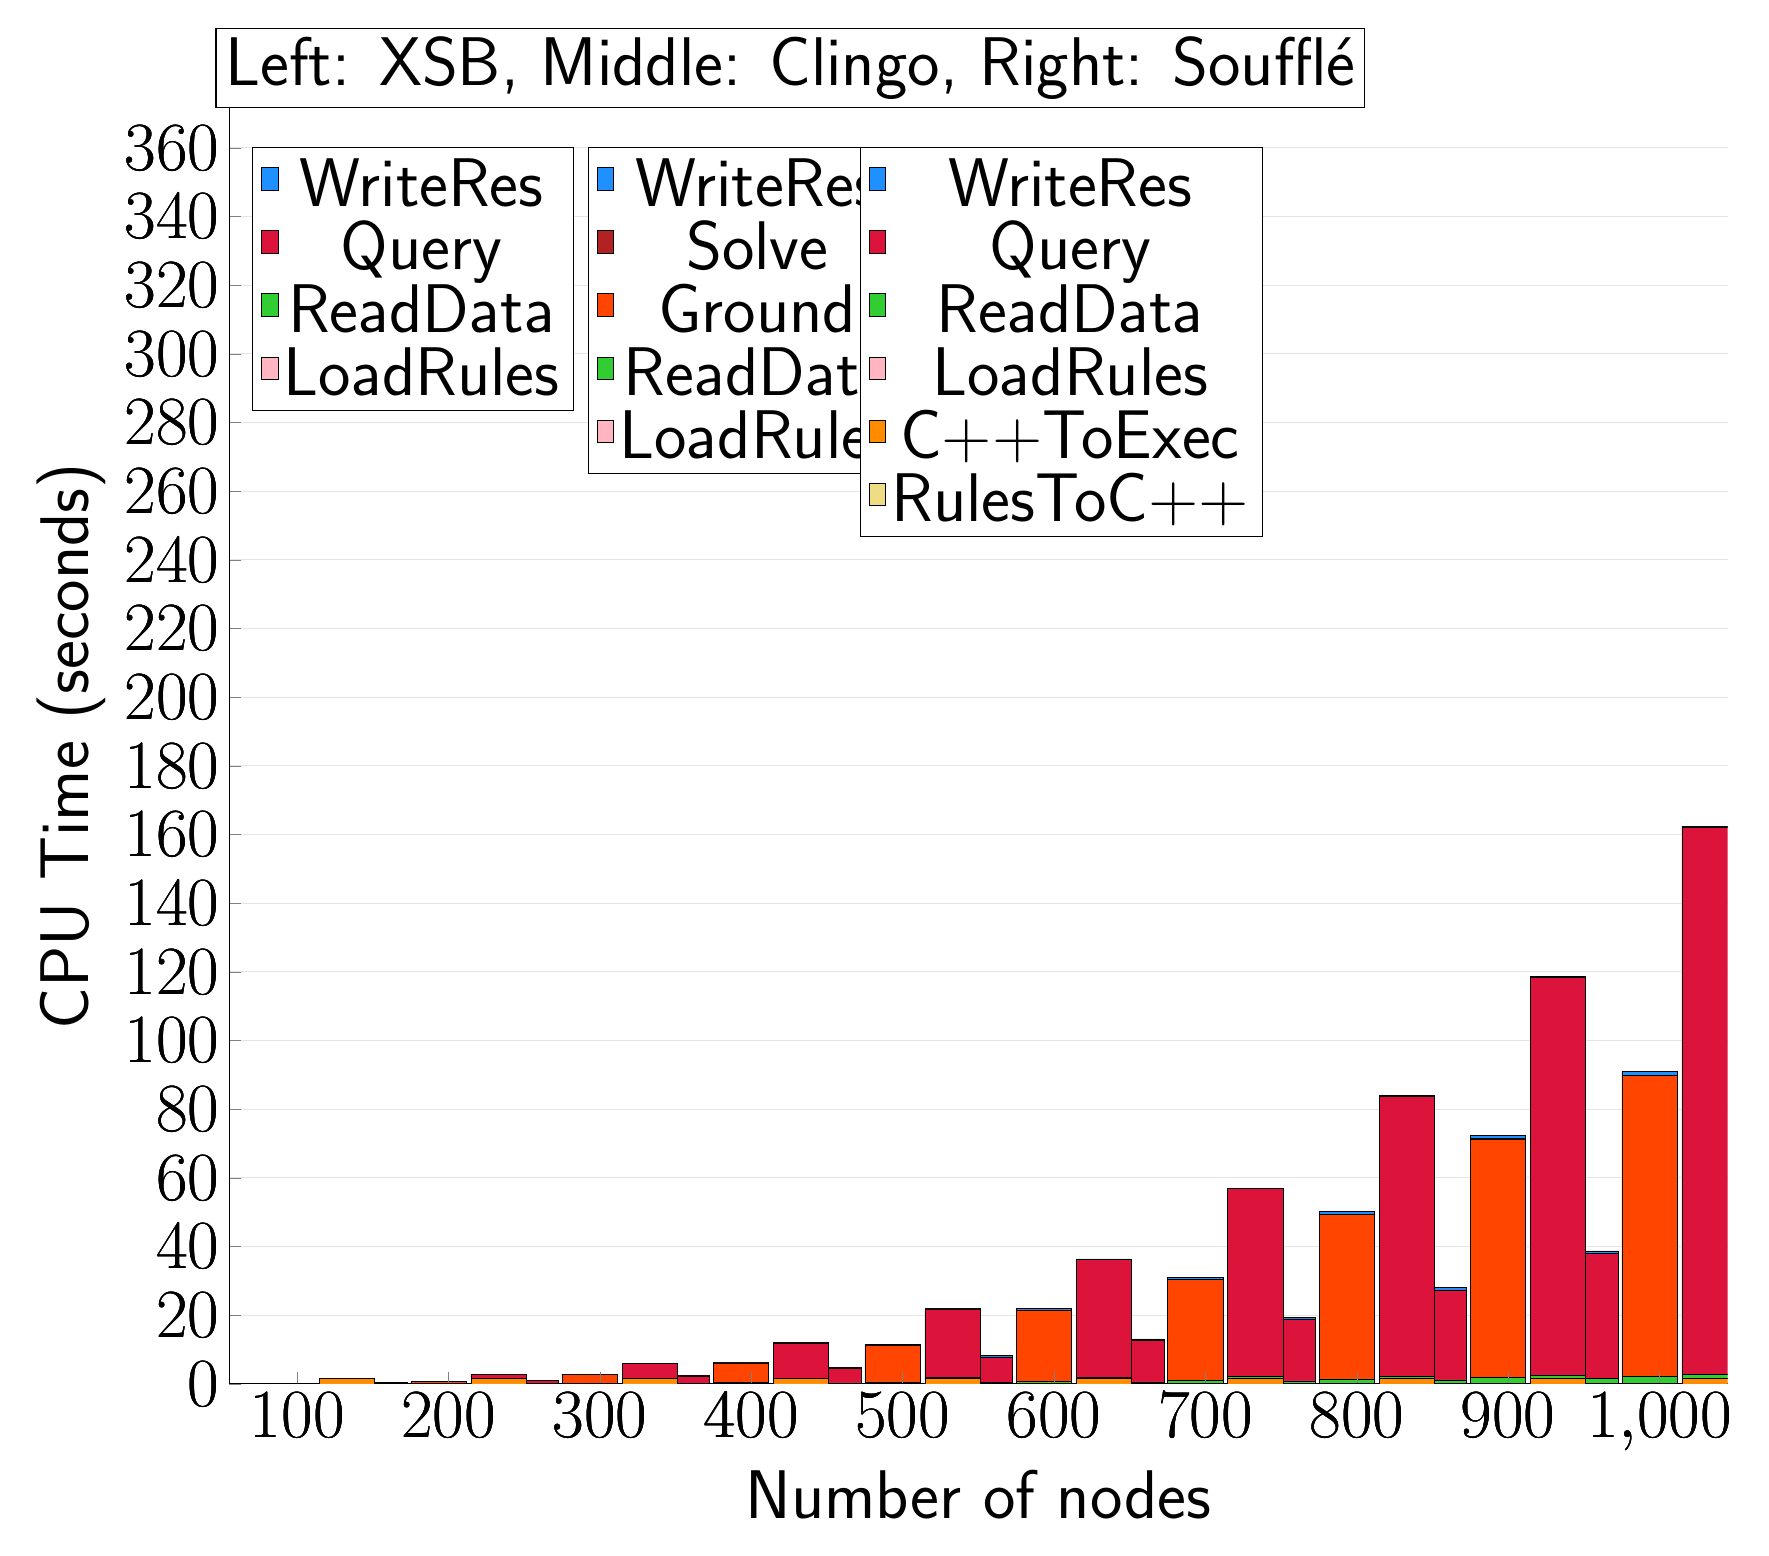
\begin{tikzpicture}
                        \begin{axis}[bar shift=-25pt, 
   ybar stacked,
   width=1.7\textwidth,
   bar width=0.7cm,
   ymajorgrids, tick align=inside,
   major grid style={draw=gray!20},
   xtick=data,
   ymin=0, ymax=371.479,
   axis x line*=bottom,
   axis y line*=left,
   enlarge x limits=0.05,
   legend style={
       at={(0.23, 0.97)},
       anchor=north east,
       legend columns=1,
       font=\Huge,
   },
   ylabel={CPU Time (seconds)},
   xlabel={Number of nodes},
   label style={font=\Huge},
   tick label style={font=\Huge},
]
\addlegendimage{fill=DodgerBlue, draw=black, line width=0.2pt}
\addlegendentry{WriteRes}
\addlegendimage{fill=Crimson, draw=black, line width=0.2pt}
\addlegendentry{Query}
\addlegendimage{fill=LimeGreen, draw=black, line width=0.2pt}
\addlegendentry{ReadData}
\addlegendimage{fill=LightPink, draw=black, line width=0.2pt}
\addlegendentry{LoadRules}
\addplot +[fill=LightPink, draw=black, line width=0.2pt] coordinates {
(100, 0.0005202000000000006)
(200, 0.0005156000000000003)
(300, 0.0005490000000000002)
(400, 0.0005499999999999998)
(500, 0.0005519999999999993)
(600, 0.0005479999999999998)
(700, 0.0005471999999999997)
(800, 0.0005578)
(900, 0.0005498000000000002)
(1000, 0.0005486000000000002)
};
\addplot +[fill=LimeGreen, draw=black, line width=0.2pt] coordinates {
(100, 0.007930399999999999)
(200, 0.034344)
(300, 0.0852434)
(400, 0.1641998)
(500, 0.26828939999999996)
(600, 0.4084958)
(700, 0.5941561999999999)
(800, 0.8269388)
(900, 1.1227968000000002)
(1000, 1.5022697999999999)
};
\addplot +[fill=Crimson, draw=black, line width=0.2pt] coordinates {
(100, 0.032986)
(200, 0.2747874)
(300, 0.9006912)
(400, 2.1476002000000003)
(500, 4.3841698000000004)
(600, 7.4668437999999995)
(700, 12.0853802)
(800, 18.062993)
(900, 26.230853000000003)
(1000, 36.4992788)
};
\addplot +[fill=DodgerBlue, draw=black, line width=0.2pt] coordinates {
(100, 0.0082554)
(200, 0.03157119999999999)
(300, 0.0723802)
(400, 0.126267)
(500, 0.2038684)
(600, 0.3009918000000001)
(700, 0.3993293999999999)
(800, 0.5169109999999989)
(900, 0.7523183999999994)
(1000, 0.741245400000001)
};
\end{axis}

\begin{axis}[bar shift=-3.7pt, 
   ybar stacked,
   width=1.7\textwidth,
   bar width=0.7cm,
   ymajorgrids, tick align=inside,
   major grid style={draw=none},
   xtick=data,
   ymin=0, ymax=371.479,
   axis x line*=none,
   axis y line*=none,
   enlarge x limits=0.05,
   legend style={
       at={(0.454, 0.97)},
       anchor=north east,
       legend columns=1,
       font=\Huge,
   },
   label style={font=\Huge},
   tick label style={font=\Huge},
]
\addlegendimage{fill=DodgerBlue, draw=black, line width=0.2pt}
\addlegendentry{WriteRes}
\addlegendimage{fill=FireBrick, draw=black, line width=0.2pt}
\addlegendentry{Solve}
\addlegendimage{fill=OrangeRed, draw=black, line width=0.2pt}
\addlegendentry{Ground}
\addlegendimage{fill=LimeGreen, draw=black, line width=0.2pt}
\addlegendentry{ReadData}
\addlegendimage{fill=LightPink, draw=black, line width=0.2pt}
\addlegendentry{LoadRules}
\addplot +[fill=LightPink, draw=black, line width=0.2pt] coordinates {
(100, 0.0)
(200, 0.0)
(300, 0.0)
(400, 0.001999999999999996)
(500, 0.0)
(600, 0.0)
(700, 0.0)
(800, 0.0)
(900, 0.0)
(1000, 0.0)
};
\addplot +[fill=LimeGreen, draw=black, line width=0.2pt] coordinates {
(100, 0.022000000000000013)
(200, 0.08000000000000002)
(300, 0.19)
(400, 0.33999999999999997)
(500, 0.544)
(600, 0.798)
(700, 1.082)
(800, 1.4300000000000002)
(900, 1.7759999999999998)
(1000, 2.268)
};
\addplot +[fill=OrangeRed, draw=black, line width=0.2pt] coordinates {
(100, 0.08999999999999997)
(200, 0.686)
(300, 2.552)
(400, 5.768)
(500, 10.542000000000002)
(600, 20.738)
(700, 29.398000000000003)
(800, 47.95)
(900, 69.56400000000001)
(1000, 87.584)
};
\addplot +[fill=FireBrick, draw=black, line width=0.2pt] coordinates {
(100, 0.0)
(200, 0.0020000000000000018)
(300, 0.007999999999999919)
(400, 0.009999999999999964)
(500, 0.01999999999999962)
(600, 0.02400000000000091)
(700, 0.032000000000000736)
(800, 0.04200000000000057)
(900, 0.05599999999999715)
(1000, 0.06400000000000046)
};
\addplot +[fill=DodgerBlue, draw=black, line width=0.2pt] coordinates {
(100, 0.01200000000000001)
(200, 0.04800000000000004)
(300, 0.10000000000000009)
(400, 0.18800000000000008)
(500, 0.2840000000000001)
(600, 0.4239999999999986)
(700, 0.5739999999999986)
(800, 0.7419999999999998)
(900, 0.9160000000000045)
(1000, 1.1480000000000015)
};
\end{axis}

\begin{axis}[bar shift=18pt, 
   ybar stacked,
   width=1.7\textwidth,
   bar width=0.7cm,
   ymajorgrids, tick align=inside,
   major grid style={draw=none},
   xtick=data,
   ymin=0, ymax=371.479,
   axis x line*=none,
   axis y line*=none,
   enlarge x limits=0.05,
   legend style={
       at={(0.69, 0.97)},
       anchor=north east,
       legend columns=1,
       font=\Huge,
   },
   label style={font=\Huge},
   tick label style={font=\Huge},
]
\addlegendimage{fill=DodgerBlue, draw=black, line width=0.2pt}
\addlegendentry{WriteRes}
\addlegendimage{fill=Crimson, draw=black, line width=0.2pt}
\addlegendentry{Query}
\addlegendimage{fill=LimeGreen, draw=black, line width=0.2pt}
\addlegendentry{ReadData}
\addlegendimage{fill=LightPink, draw=black, line width=0.2pt}
\addlegendentry{LoadRules}
\addlegendimage{fill=DarkOrange, draw=black, line width=0.2pt}
\addlegendentry{C++ToExec}
\addlegendimage{fill=LightGoldenrod, draw=black, line width=0.2pt}
\addlegendentry{RulesToC++}
\addplot +[fill=LightGoldenrod, draw=black, line width=0.2pt] coordinates {
(100, 0.008000000000000002)
(200, 0.004000000000000001)
(300, 0.008000000000000002)
(400, 0.0020000000000000005)
(500, 0.0020000000000000005)
(600, 0.0020000000000000005)
(700, 0.0)
(800, 0.0)
(900, 0.0)
(1000, 0.0)
};
\addplot +[fill=DarkOrange, draw=black, line width=0.2pt] coordinates {
(100, 1.472)
(200, 1.482)
(300, 1.482)
(400, 1.4899999999999998)
(500, 1.488)
(600, 1.4760000000000002)
(700, 1.4819999999999998)
(800, 1.482)
(900, 1.474)
(1000, 1.476)
};
\addplot +[fill=LightPink, draw=black, line width=0.2pt] coordinates {
(100, 0.0001718)
(200, 0.0001714)
(300, 0.0001638)
(400, 0.0001738)
(500, 0.00016479999999999997)
(600, 0.00019319999999999998)
(700, 0.000191)
(800, 0.0001898)
(900, 0.000203)
(1000, 0.00019940000000000002)
};
\addplot +[fill=LimeGreen, draw=black, line width=0.2pt] coordinates {
(100, 0.025143200000000004)
(200, 0.0683648)
(300, 0.1247746)
(400, 0.20489039999999997)
(500, 0.30804580000000004)
(600, 0.43432780000000004)
(700, 0.5867352)
(800, 0.757899)
(900, 0.9560248)
(1000, 1.1800599999999999)
};
\addplot +[fill=Crimson, draw=black, line width=0.2pt] coordinates {
(100, 0.1748882)
(200, 1.288402)
(300, 4.312656)
(400, 10.2421)
(500, 20.02474)
(600, 34.37328)
(700, 54.81555999999999)
(800, 81.53943999999998)
(900, 115.973)
(1000, 159.53879999999998)
};
\addplot +[fill=DodgerBlue, draw=black, line width=0.2pt] coordinates {
(100, 0.0023746)
(200, 0.0089314)
(300, 0.019713)
(400, 0.034501)
(500, 0.054256799999999994)
(600, 0.0779796)
(700, 0.10419199999999999)
(800, 0.1352344)
(900, 0.1724408)
(1000, 0.2128844)
};
\end{axis}


\node[anchor=south, draw, fill=white] at (rel axis cs:0.42,1) {\Huge Left: XSB, Middle: Clingo, Right: Soufflé};
\end{tikzpicture}
\end{document}
                    